% cd /disks/PROJECT/Mickael/COMMUNICATION/CST2016/;
% pdflatex THESE_CST2016.tex; bibtex THESE_CST2016; pdflatex THESE_CST2016.tex; pdflatex THESE_CST2016.tex;
% evince THESE_CST2016.pdf &

\documentclass[11pt, a4paper]{article}
\input{Header_Article.tex}
\usepackage{eso-pic}
\usepackage{transparent}
\AddToShipoutPicture*{\AtPageLowerLeft{\transparent{0.30}
\includegraphics[width=\paperwidth,height=\paperheight]{figures/BG03_A0.jpg}}}

\usepackage{pdfpages}

\usepackage[english, francais]{babel}
\selectlanguage{francais}

\addto\captionsfrancais{%
   \def\figurename{Figure}%
}
\addto\captionsfrancais{%
   \def\tablename{Table}%
}

\title{\huge{Développement et Application de Méthodologies Statistiques pour Etudes Longitudinales d'Association Génétique}\linebreak \large{\textit{Comité de Suivi de Thèse: deuxième année}}}
\date{26 septembre 2016}
\email{\href{mailto:mickael.canouil@cnrs.fr}{mickael.canouil@cnrs.fr}}
\author{Mickaël Canouil}
\grade{Doctorant en Biostatistique}
\institute{\cmdb{G}énomique \cmdb{I}ntégrative et \cmdb{M}odélisation des \cmdb{M}aladies \cmdb{M}étaboliques \linebreak UMR 8199 (CNRS / Université de Lille 2 / Institut Pasteur de Lille)}
\address{CNRS UMR 8199 - Institut de Biologie de Lille\linebreak
1 Rue du Professeur Calmette\linebreak
BP 245\linebreak
F-59019 LILLE CEDEX
}
\cst{
\textbf{Directeur de thèse:}\\ Pr. Philippe Froguel\\ \vskip 0.25cm
\textbf{Co-directeur de thèse:}\\ Dr. Ghislain Rocheleau (Lille 2)\\ \vskip 0.25cm
\textbf{Membres du CST:}\\ Dr. Hélène Jacqmin-Gadda (INSERM U 897, Bordeaux)\\
Pr. Cristian Preda (Ecole Polytechnique, Lille)
}

% <<title, echo = FALSE, results = hide>>=
% @


\begin{document}
\maketitle
\tableofcontents

\clearpage
\section{Introduction et contexte}
\par{La prévalence mondiale du diabète de type 2 (DT2) est en constante augmentation et induit de ce fait la recherche de nouveaux marqueurs génétiques impliqués dans le risque de survenue de la maladie \citep{world_health_organization_diabetes_2015}.
Ces dernières années, les études d’association pangénomique (GWAS) ont identifié 65 loci associés à la susceptibilité au DT2 \citep{morris_large-scale_2012}.
Les GWAS ont notamment identifié 36 variants associés à la glycémie à jeun chez des individus normoglycémiques \citep{dupuis_new_2010, scott_large-scale_2012}.
Bien que le rôle fonctionnel de la plupart de ces loci reste à déterminer, ils ont tout de même permis de mettre en lumière des liens intéressants entre la concentration de glucose sanguin et le DT2,
et souligné quelques différences entre l’homéostasie du glucose dans la population générale et les niveaux physiopathologiques observés chez les diabétiques.
La majorité de ces loci ont été trouvés par une  méta-analyse de GWAS, malgré la très grande hétérogénéité des études et des cohortes incluses dans la méta-analyse.}

\par{La grande majorité des GWAS publiées a utilisé un design transversal plutôt qu’un design longitudinal.
Cependant, une étude prospective longitudinale offre la possibilité de mesurer une même variable plusieurs fois au cours de l’étude, permettant également une description de ses fluctuations temporelles.
La  puissance permettant de détecter des variants génétiques associés à ces variables devrait être augmentée grâce aux multiples mesures prises à plusieurs moments,
puisqu’elles donnent globalement plus d’informations qu’une seule mesure prise à un moment donné.
De plus, un design longitudinal permet d’étudier les variants associés aux changements (trajectoires) de ces mesures à travers le temps,
tout en augmentant la puissance permettant  de détecter des différences entre les groupes (définis par leur génotype, dans un contexte génétique).
Tout porte à croire qu’une bonne modélisation de ces trajectoires optimiserait les tests d’association et permettrait une meilleure exploitation des phénotypes disponibles.}


\clearpage
\section{Objectif de la thèse}
\par{Cette thèse propose de développer et implémenter des approches pangénomiques basées sur des modèles de régression, tels les modèles linéaires mixtes (LMM), les équations estimantes généralisées (GEE) \citep{sitlani_generalized_2015},
et les modèles joints (JM) liant de façon statistique la variation temporelle d’une variable (p.ex. le glucose sanguin à jeun FG) avec la survenue d’une maladie (p.ex. le DT2).
Ces approches pourraient mener à l’identification de nouveaux loci.
De plus, ces méthodologies permettront de confronter la vision actuelle,
selon laquelle les gènes impliqués dans le contrôle de la glycémie chez les individus normoglycémiques diffèrent de ceux observés chez les individus atteints de DT2 \citep{yaghootkar_recent_2013}.
Aussi, ces approches statistiques appliquées à un contexte génétique pourraient permettre d’expliquer pourquoi certains individus en légère hyperglycémie ne développent pas de DT2.
Les marqueurs ainsi identifiés renforceront du même coup l’utilité clinique de la stratification génétique du risque dans la population générale \citep{pal_genetics_2013}.}

\par{Néanmoins, les approches LMM, GEE et JM nécessitent de grandes quantités de ressources informatiques lorsqu’appliquées sur des millions de loci et des milliers d’individus.
Ces approches sont le plus souvent utilisées sur un sous-ensemble de loci dans des régions d’intérêts de la pathologie étudiée \citep{beyene_longitudinal_2014, wu_longitudinal_2014}.
Des approches dites "rapides" ont été développées pour pallier au problème du temps de calcul, présents notamment sur les
implémentations actuelles des LMM (\cmd{nlme} et \cmd{lme4} pour R), et se basent sur des méthodes
d’approximation des LMM \citep{sikorska_fast_2013, sikorska_gwas_2015, sikorska_computationally_2014}.
A ce jour, deux implémentations des JM existent sur la plateforme CRAN pour le logiciel R \citep{Rsoftware}.
La première est développée par Dimitris Rizopoulos (\cmd{JM}) \citep{rizopoulos_jm_2010} et la seconde est développée par Pete Philipson (\cmd{joineR}) \citep{philipson_joiner_2012}.}

\par{La cohorte prospective D.E.S.I.R (Données Épidémiologiques sur le Syndrome d’Insulino-Résistance)\citep{balkau_epidemiologic_1996},
comprend 5~212 individus suivis pendant neuf années au cours desquelles plusieurs mesures
phénotypiques ont été prises à quatre occasions uniformément réparties durant la période de suivi (0, 3, 6 et 9 ans).
En exploitant l’approche par GWAS dans la cohorte D.E.S.I.R, une percée majeure a été réalisée dans la génétique
des traits métaboliques menant, d’une part, à la découverte de nouveaux loci associés au DT2, et d’autre part,
à l’identification de loci impliqués dans la contrôle de la glycémie d’individus normoglycémiques \citep{dupuis_new_2010, voight_twelve_2010}.
La base de données phénotypiques et génotypiques existante de D.E.S.I.R offre l’opportunité unique de modéliser
la trajectoire temporelle de plusieurs phénotypes dont la glycémie à jeun, et peut-être même permettra
de découvrir de nouveaux loci simultanément associés à l’incidence du DT2 et à un taux élevé de glucose sanguin.}
\par{L’étude des données a été réalisée avec le logiciel R sur un serveur de calcul de 80 coeurs
et 500 Go de mémoire vive, accessible dans le laboratoire de l'unité UMR 8199 dirigée par le Pr. Philippe Froguel.}


\clearpage
\section{Données phénotypiques et génotypiques\label{sec:Materiels}}
\par{Le génotypage a été réalisé à l'aide de la puce MetaboChip (Infinium iSelect Custom Genotyping Arrays)\citep{voight_metabochip_2012},
via la technologie Illumina HiScan et le logiciel GenomeStudio (Illumina, San Diego, CA, 19 USA),
pour ..
Les individus de cette cohorte ont été suivis pendant neuf ans, où des données phénotypiques ont été recueillies à différentes occasions: à l'inclusion, trois ans, six ans et neuf ans.
Le contrôle qualité a été réalisée au moyen du logiciel PLINK (1.90 beta)\citep{chang_second-generation_2015, purcell_plink_2015}.}
\par{Un "call rate" (qualité du génotypage) de 95\% a été utilisé pour filtrer aussi bien les individus que les SNPs (Single Nucleotide Polymorphism),
de même seuls les SNPs ne présentant pas de déviation à l'équilibre de Hardy-Weinberg ($p<1 \times 10^{-3}$) et dont la fréquence de l'allèle mineur
était supérieure à 1\% ont été conservés, soit 124~095 SNPs et 4~884 individus.}
\par{Une analyse en composantes principales a été réalisée sur un jeu de données combinant les 4~884 individus de la cohorte D.E.S.I.R.
et les 2~504 individus disponibles dans la base de données publique du projet 1~000 Génomes \citep{the_1000_genomes_project_consortium_global_2015},
et réduit aux SNPs présents dans les deux jeux de données et non palindromique (107~591 SNPs).
Le premier plan factoriel était suffisant pour discriminer l'origine ethnique des individus et a permis de réduire le nombre d'individus à 4~565 individus Caucasiens.
De plus, 86 individus ont été exclus, en raison de phénotypes manquants (sexe, Indice de masse Corporelle, glycémie à jeun), ne permettant pas d'établir le statut DT2 de ces individus.
Les cas prévalents de DT2 (glycémie supérieure à $7mmol/L$ ont également été retirés de l'analyse (115 individus).}
\par{Le jeu de données final utilisé pour les analyses incluait 4~364 individus (dont 179 DT2 incidents) et 124~095 SNPs.}


\clearpage
\section{Méthodes\label{sec:Methods}}
\subsection{Modèle Joint}
\begin{figure}[ht]
    \begin{center}
        \fbox{\includegraphics[width=7.5cm]{figures/jointModel.png}}
    \end{center}
    \vspace{-15pt}
    \captionof{figure}{Diagramme général d'un modèle joint pour le T2D (adapté de \cite{ibrahim_basic_2010})\newline
    {\small $X(t)$: trajectoire de la glycémie à jeun inférée des données longitudinales observées;
    $\alpha$: effet du SNP sur le diabète;
    $\gamma$: effet du SNP sur la trajectoire de la glycémie à jeun;
    $\beta$: effet de la trajectoire de la glycémie à jeun sur le diabète.}}
    \label{fig:JointModel}
\end{figure}
\par{En utilisant, l'approche de modèle joint implémentée dans l'extension JM \citep{rizopoulos_jm_2010} du logiciel R (version 3.2.3)\citep{r_core_team_r_2015},
124~095 SNPs de la MetaboChip ont été testés simultanément pour leur association avec la glycémie à jeun et le risque de DT2.}

\par{La formulation standard du modèle joint implique deux composantes, d'une part, une composante longitudinale pour modéliser la trajectoire de la variable étudiée,
et d'autre part, une composante de survie pour modéliser la survenue de l'événement étudié.
La composante longitudinale consiste typiquement à l'application d'un modèle linéaire mixte:
\begin{eqnarray}Y_{ij}=X_{ij}+\epsilon_{ij},\label{eq:1}\end{eqnarray}
où $Y_{ij}$ est la valeur observée et $X_{ij}$ la vraie (non-observée) valeur de la variable longitudinale.
Le terme $\epsilon_{ij}$ est le terme d'erreur aléatoire supposé être distribué selon la Loi Normale:
\begin{eqnarray}\epsilon_{ij} \sim \mathcal{N}(0, \sigma^2)\label{eq:2}\end{eqnarray}
La quantité $X_{ij}$ (ou $X(t)$) est la fonction de la trajectoire et est définie usuellement comme une fonction linéaire (ou quadratique) du temps $t$.}

\par{Des covariables peuvent être incluses dans la fonction de la trajectoire, comme l'âge, le sexe ou l'IMC.
Dans notre étude, $Y_{ij}$ représente les valeurs mesurées la glycémie à jeun au temps $t_{ij}$, $Z_i$ désigne le génotype du SNP analysé pour l'individu $i$ et $W_i$ désigne les covariables selon le modèle suivant:
\begin{eqnarray}Y_{ij}=X_{ij}+\epsilon_{ij}=\theta_{0i}+\theta_{1i}\times t_{ij}+\gamma \times Z_i+\delta \times W_i + \epsilon_{ij}\label{eq:3}\end{eqnarray}
Pour simplifier, le terme $\delta \times W_i$ sera omis dans la suite.}

\par{Les paramètres $\theta_{0i}$ et $\theta_{1i}$ sont supposés être distribués selon une distribution normale multivariée:
\begin{eqnarray}\boldsymbol\theta \sim \mathcal{N}_2(\boldsymbol\mu, \boldsymbol\Sigma)\label{eq:4}\end{eqnarray}
Le paramètre $\gamma$ évalue l'effet additif du SNP ($Z_i$) sur la fonction de la trajectoire.
Pour tenir compte éventuellement de pentes variant entre les génotypes, un terme d'interaction entre le SNP et le temps peut être inclus dans la fonction de la trajectoire.
Le terme d'interaction n'a pas été inclus dans notre étude.}

\par{La composante de survie (survenue du DT2) se compose généralement d'un modèle paramétrique (p.ex. exponentielle ou Weibull) ou semi-paramétrique (p.ex. risques proportionnels de Cox) avec:
\begin{eqnarray}h_i(t)=h_0(t) exp(\beta X_i(t)+\alpha Z_i),\label{eq:5}\end{eqnarray}
où $h_i(t)$ est la fonction de risque au temps $t$ pour l'individu $i$ et $h_0(t)$ est la fonction de risque de base non spécifiée, supposée être une constante par morceaux avec deux noeuds placés à des temps intermédiaires
(c'est-à-dire, à trois et six ans sur les neuf ans du suivi). Le coefficient $\alpha$ mesure l'effet du SNP sur le délai d'apparition du DT2,
alors que le coefficient $\beta$ mesure l'association entre la trajectoire du niveau de la glycémie à jeun et le temps d'apparition du DT2.}

\clearpage
\subsection{Simulation}
\par{Des études de simulation ont été menées pour examiner la puissance statistique et l'erreur de type 1 des SNPs trouvés comme nominalement associé (à 5\%) en utilisant le modèle joint, comme implémenté par \citet{rizopoulos_jm_2010}.
Notre objectif principal était de déterminer le gain ou la perte de puissance du modèle joint par rapport aux approches classiques transversales (p.ex. régression logistique ou linéaire, modèle de Cox)
pour détecter l'effet d'un SNP, sur la glycémie à jeun et le statut DT2 dans notre étude.
Les jeux de données de simulation, qui ont été réalisés avec R, suivent les \hyperref[eq:1]{Equations~\ref*{eq:1}~à~\ref{eq:5}},
avec la fonction de risque de base fixée ($h_0(t)=\lambda$) de façon à obtenir une incidence équivalente à celle de la cohorte D.E.S.I.R (environ 5\%), durant la période de suivi de neuf ans.
Les temps d'événements ont été générés selon une distribution exponentielle dans le cadre du modèle de Cox à risque proportionnel \citep{austin_generating_2012}.
\begin{eqnarray}H(T)=\int_0^T \lambda exp(\beta \times X(t) + \alpha \times Z) dt\end{eqnarray}
\begin{eqnarray}T=\frac{1}{\beta\theta_1} log\left( - \frac{\beta\theta_1 \times log(1-u)}{\lambda exp(\beta\theta_0+(\beta\gamma+\alpha)Z)}+1 \right)\end{eqnarray}
}

\subsection{Puissance statistique}
\par{La puissance statistique a été calculée, 1) au niveau du modèle joint, à l'aide de la formule de \citet{chen_sample_2011}:
\begin{eqnarray}z_{\tilde{\beta}}=&\pm\sqrt{Df(1-f)(\beta\gamma+\alpha)^2}+z_{1-\tilde{\alpha}/2},\end{eqnarray}
avec $D$, le nombre de DT2 incidents et $f$, la fréquence de l'allèle à risque,
2) au niveau des paramètres $\gamma$ et $\alpha$ respectivement pour l'effet du SNP sur la trajectoire de la glycémie à jeun et sur le risque de DT2.}


\clearpage
\section{Résultats d'application}
\begin{figure}[ht]
    \begin{center}
        \fbox{\includegraphics[width=15cm]{figures/Yaghootkar.png}}
        \captionof{figure}{Résultat d'association des allèles à risque pour le T2D et/ou la glycémie à jeun par GWAS \citep{yaghootkar_recent_2013}.
        \textcolor{dodgerblue}{Cercle bleu}: l'association à la glycémie à jeun pour $\textrm{p}<5\times 10^{-8}$;
        \textcolor{firebrick2}{Triangle rouge}: l'association au T2D et à la glycémie à jeun $\textrm{p}<5\times 10^{-8}$.}
        \label{fig:gwas}
    \end{center}
\end{figure}
\par{Les approches classiques de GWAS ont pu mettre en évidence entre 80 et 100 loci associés au DT2 et au FG, notamment via des méta-analyses \citep{yaghootkar_recent_2013, dupuis_new_2010, vaxillaire_type_2014},
dont certains de ces loci (gènes) sont montrés sur la \bref{fig:gwas}{Figure}.}
\par{Dans le cadre des données génotypiques et phénotypiques disponibles dans la cohorte D.E.S.I.R. (\bref{sec:Materiels}{Section}),
nous avons analysé l'ensemble des 124~095 SNPs disponibles à l'aide d'un modèle joint (\bref{sec:Methods}{Section}),
nous permettant ainsi d'identifier 145 loci associés à la fois à la trajectoire de la glycémie à jeun et également à la survenue du DT2 (au seuil statistique de 5\%).
Ces loci sont présentés dans la \bref{fig:results}{Figure}, avec la puissance calculée selon les formules développées par \citet{chen_sample_2011}.}

\begin{figure}[h]
    \begin{center}
        \fbox{\includegraphics[width=15cm]{/disks/DATA/DESIR_longitudinal/16-JointModel_MetaboChipSimu/CST2016_Figure2.png}}
        \captionof{figure}{Résultat d'association des allèles à risque pour le T2D et/ou la glycémie à jeun à partir du modèle joint.}
        \label{fig:results}
    \end{center}
\end{figure}
\par{Parmi les 145 loci obtenus, 13 ont déjà été identifiés dans des GWAS \citep{welter_nhgri_2014} pour être associés à la glycémie à jeun et/ou au DT2.
Les 132 loci restants ne pourraient être que des faux positifs en raison du seuil peu stringent utilisé ici (5\%) et du nombre de tests effectués (124~095).
Ainsi, une validation de ces résultats devra être effectués à l'aide d'une cohorte de réplication par exemple.}

\par{Cependant, au regard des résultats obtenus par l'approche de modélisation jointe de la trajectoire de la glycémie à jeun et la survenue du DT2,
notamment au niveau des 13 loci répertoriés dans le GWAS catalog \citep{welter_nhgri_2014} (\bref{tab:tab1}{Table} et \bref{fig:results}{Figure}),
nous pouvons noter des effets cohérents par rapport à ceux reportés dans la littérature.
À cela, le gène MTNR1B fait exception, comme le montre la localisation de ce gène sur la \bref{fig:gwas}{Figure} et la \bref{fig:results}{Figure}, suggérant un effet opposé sur le risque de survenue du DT2 au cours du suivi.
En effet, MTNR1B a été reporté, notamment par \citet{bouatia-naji_variant_2009} et \citet{lyssenko_common_2009} comme associé à une élévation de la glycémie et une augmentation du risque de DT2.
Ce phénomène pourrait être expliqué par une certaine spécificité de la cohorte, puisque le gène MTNR1B a été identifié via méta-analyse.
D'autre part, comme le souligne Dr. Dimitris Rizopoulos \citep{rizopoulos_joint_2012}, les cas incidents de DT2 pourraient ne pas être homogènes de par leurs caractéristiques cliniques et plus généralement phénotypiques.}
\newpage
\begin{bquote}{Dimitris Rizopoulos}
In some occasions the typical assumption that the current value of the timedependent covariate affects the current risk for an event may lead to medically
illogical conclusions. For example, this has been observed by Cavender et al. (1992) who in a study on patients with coronary artery disease noted that the
current smoking status decreased the risk for death (although not statistically significantly). The reason behind this surprising result was that most of those
who died were smokers, but many had stopped smoking at the last follow-up before their death. Thus, many of the patients who died had just quit smoking,
whereas some of the patients who were still alive were still smoking, leading to the surprising result.
\end{bquote}
\par{Une approche dites à classes latentes pourrait être utilisée \citep{proust-lima_joint_2009} pour prendre en compte une possible hétérogénéité dans la population et ainsi pourrait permettre d'expliquer le résultat obtenu pour le gène MTNR1B.}
\begin{table}[h]
    \begin{center}
        {\small\input{"/disks/DATA/DESIR_longitudinal/16-JointModel_MetaboChipSimu/CST2016_Table1.tex"}}
        \captionof{table}{Résultat d'analyse pour une sélection de SNPs connus pour être associés au T2D et/ou à la glycémie à jeun.
        {En \textcolor{dodgerblue}{bleu}: $\textrm{p}<0.05$, en \textcolor{firebrick2}{rouge}: $\textrm{p}<5\times 10^{-8}$.
        Puissance selon la formule de \citet{chen_sample_2011}.}}
        \label{tab:tab1}
    \end{center}
\end{table}
\newpage
\par{L'un des objectifs de l'utilisation d'un modèle joint, en dehors de la modélisation jointe du processus de survie et du processus longitudinal,
était de mettre à profit les mesures répétées pouvant être disponibles dans l'objectif d'accroître la puissance statistique, pour détecter un effet d'un SNP sur le ou les traits étudiés,
en comparaison des approches classiques et transversales des GWAS (\bref{tab:tab2}{Table}).}
\begin{table}[h]
    \begin{center}
        {\small\input{"/disks/DATA/DESIR_longitudinal/16-JointModel_MetaboChipSimu/CST2016_Table2.tex"}}
        \captionof{table}{Puissance statistique obtenu par simulation pour les paramètres $\alpha$ (effet du SNP sur le statut) et $\gamma$ (effet du SNP sur la trajectoire de la glycémie à jeun).
            {En \textcolor{dodgerblue}{bleu}, lorsque le modèle joint (JM) est plus puissant que le modèle transversal à un temps donné (CM), présenté sous la forme JM / CM. (Erreur de type I:  $5.81\%\pm0.83$ / $5.47\%\pm0.64$ pour JM et CM.)}}
        \label{tab:tab2}
    \end{center}
\end{table}


\clearpage
\section{Perspectives}
\par{
\begin{enumerate}
    \item Ecriture d’un rapport scientifique (Bourse SFD-Lilly: 21 Mai 2017) et d'un article sur l'application du modèle joint à la cohorte DESIR
    \item Validation des SNPs/gènes mis en évidence par le modèle joint (p.ex. cohorte de réplication)
    \item Etude d'autre trait tel que l'HbA1c (hémoglobine glyquée)
    \item Inclusion des individus incident pour l'IFG (Impaired Fasting Glucose; $FG>6.1mM/L$) en plus des individus DT2 ($FG>7mM/L$)
\end{enumerate}
}


\clearpage
\section{Formations}
\subsection{Futures}
\par{
\begin{itemize}
    \item \textit{Congrès IGES 2016} (International Genetic Epidemiology Society): Présentation poster "Single Nucleotide Polymorphisms Associated With Fasting Blood Glucose Trajectory And Type 2 Diabetes Incidence: A Joint Modelling Approach"
    \item \textit{Congrès de la SFD 2017} (Société Francophone du Diabète)
    \item \textit{Congrès de la SFdS 2017} (Société Française de Statistique)
    \item \textit{Rencontres R 2017}
    \item \textit{useR 2017}
    \item ...
\end{itemize}
}

\subsection{Passées}
\par{
Nombre de crédits obtenus à ce jour: 47/60 crédits.
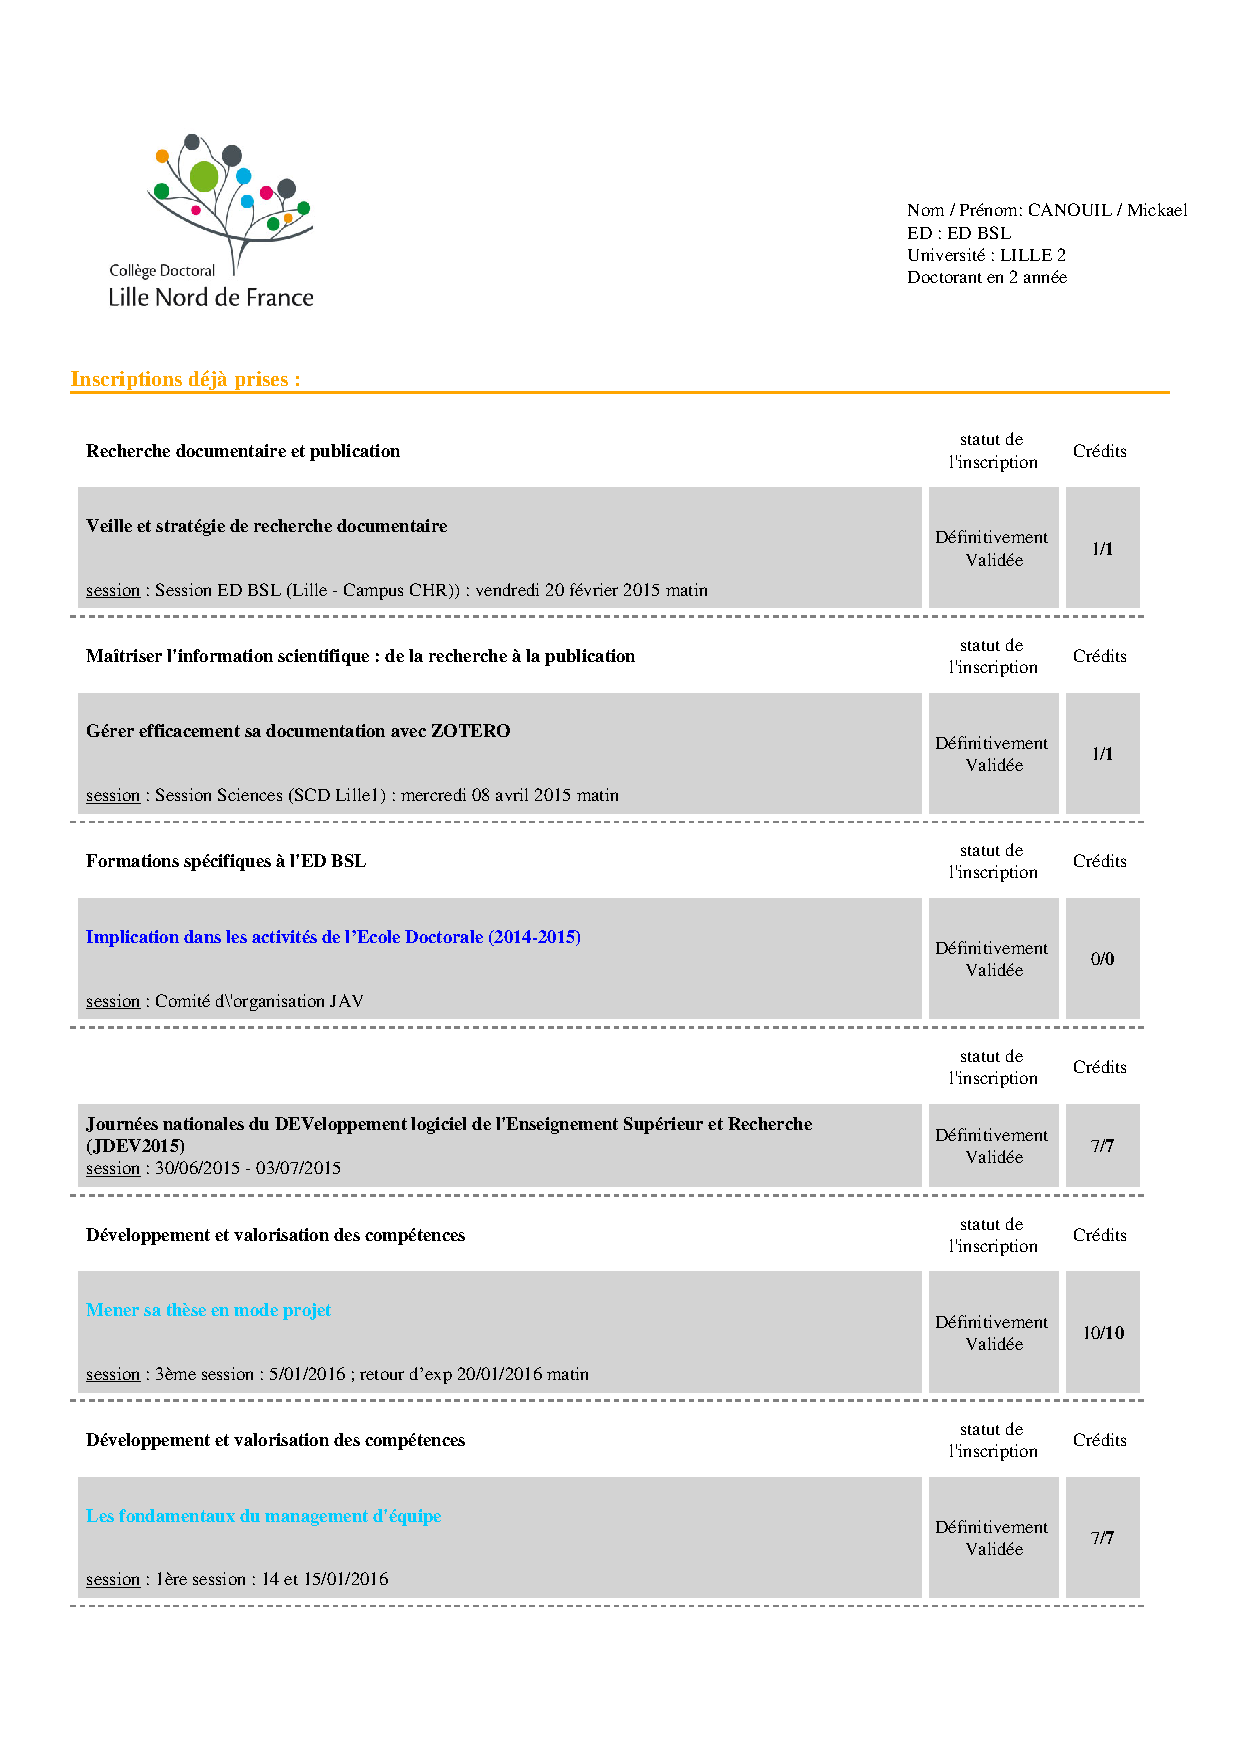
\includepdf[pages=-,scale=.8,pagecommand={}]{PortFolio2016.pdf}
}



% \setlength{\tabcolsep}{10pt} % default
\clearpage
\addcontentsline{toc}{section}{Références}
\bibliographystyle{apalike}
\bibliography{CST2016.bib}
% \nocite{*}


% \appendix
% \setcounter{table}{0}
% \setcounter{figure}{0}
% \renewcommand\thetable{\alph{table}}
% \renewcommand\thefigure{\alph{figure}}
% \clearpage

\end{document}